\begin{surferPage}[Cúspide A2++]{Otra cúspide (singularidad $A_2^{++}$)}
 Es similar a la cúspide anterior.
Su ecuación es la misma, salvo un cambio de signo:
    \vspace*{-0.4em}
    \begin{center}
      $x^3+y^2+z^2=0.$
    \end{center}
    \vspace*{-0.4em}
Este cambio da una superficie de revolución (no cambia por
giros alrededor del eje $x$), como lo es su deformación
    $(1-a)x^3-ax^2+y^2+z^2=0$, $a>0$
en una singularidad del tipo $A_1^{+-}$:
    \begin{center}
      \vspace*{-0.6em}
      \begin{tabular}{@{}c@{\quad}c@{\quad}c@{}}
        \begin{tabular}{@{}c@{}}
          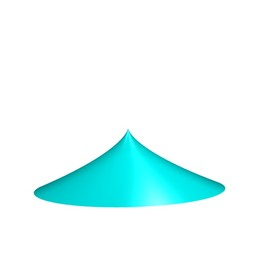
\includegraphics[width=1.2cm]{../../common/images/A2pp_0}
        \end{tabular}
        &
        \begin{tabular}{@{}c@{}}
          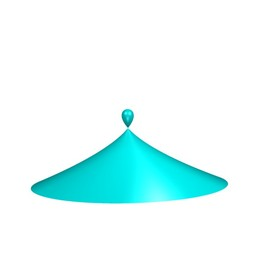
\includegraphics[width=1.2cm]{../../common/images/A2pp_1}
        \end{tabular}
        &
        \begin{tabular}{@{}c@{}}
          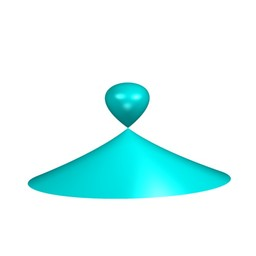
\includegraphics[width=1.2cm]{../../common/images/A2pp_2}
        \end{tabular}
      \end{tabular}
    \end{center}
    \vspace*{-0.5em}
Nótese que si escribimos la ecuación en la forma
$y^2+z^2=-(x^3)$, que muestra que para un valor fijado
$x<0$ se obtiene una circunferencia ($y^2+z^2=r^2$ representa una
circunferencia de radio $r$, por el teorema de Pitágoras).
El corte de la cúspide deformada por el plano $z=0$ da una cúspide plana
(si $a=0$) o un lazo (si $a\neq0$).
    \begin{center}
      \vspace*{-0.7em}
      \begin{tabular}{@{}c@{\quad}c@{\quad}c@{}}
        \begin{tabular}{@{}c@{}}
          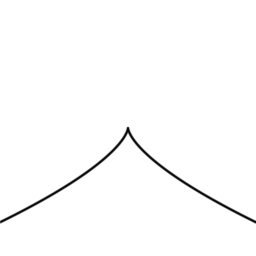
\includegraphics[width=1.2cm]{../../common/images/cuspe_def_cut_1}
        \end{tabular}
        &
        \begin{tabular}{@{}c@{}}
          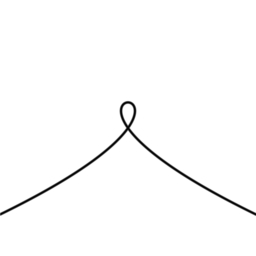
\includegraphics[width=1.2cm]{../../common/images/cuspe_def_cut_2}
        \end{tabular}
        &
        \begin{tabular}{@{}c@{}}
          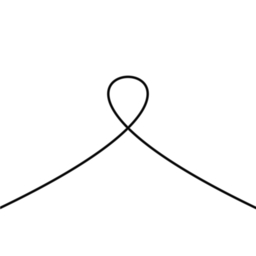
\includegraphics[width=1.2cm]{../../common/images/cuspe_def_cut_3}
        \end{tabular}
      \end{tabular}
    \end{center}
\end{surferPage}
